\documentclass[border=10pt]{standalone}
\usepackage{pgfplots}
\pgfplotsset{compat=1.18}
\begin{document}
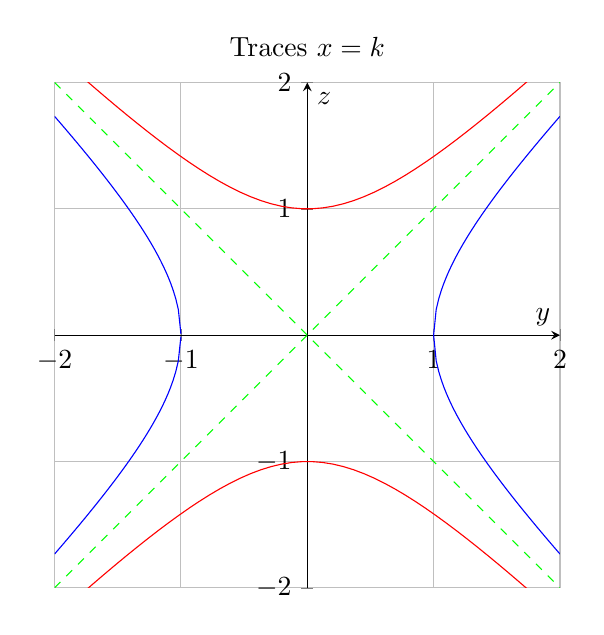
\begin{tikzpicture}
\begin{axis}[
    xlabel={$y$},
    ylabel={$z$},
    title={Traces $x=k$},
    xmin=-2, xmax=2,
    ymin=-2, ymax=2,
    axis lines=center,
    grid=major,
    width=8cm,
    height=8cm,
]
\addplot[blue, domain=1:2, samples=50] {sqrt(x^2-1)};
\addplot[blue, domain=1:2, samples=50] {-sqrt(x^2-1)};
\addplot[blue, domain=-2:-1, samples=50] {sqrt(x^2-1)};
\addplot[blue, domain=-2:-1, samples=50] {-sqrt(x^2-1)};
\addplot[red, domain=-2:2, samples=50] {sqrt(1+x^2)};
\addplot[red, domain=-2:2, samples=50] {-sqrt(1+x^2)};
\addplot[green, dashed, domain=-2:2, samples=2] {x};
\addplot[green, dashed, domain=-2:2, samples=2] {-x};
\end{axis}
\end{tikzpicture}
\end{document}